\documentclass{article}
\usepackage[a4paper, total={6in, 8in}]{geometry}
\usepackage[utf8]{inputenc}
\usepackage{algorithm} 
\usepackage{algpseudocode}
\usepackage{graphicx}
%\graphicspath{ {images/} }
\usepackage[rightcaption]{sidecap}

\usepackage{wrapfig}



\title{CS345 Special Assignment Report}
\author{Raktim Mitra(150562) \\
    Pranjal Prasoon(150508)}
\date{13 October 2017}
\begin{document}
\maketitle
\newpage
\section*{Running Time of Brute force algorithm:}
\begin{figure}[th]%
\centering

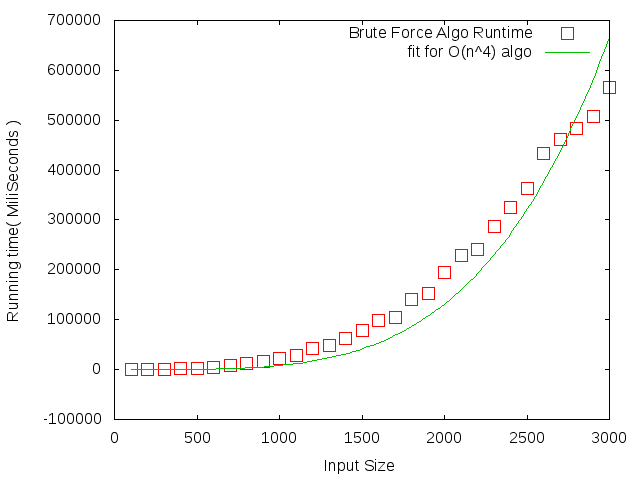
\includegraphics[width=0.5\columnwidth]{brute1.png}%
\caption{Runtime vs Input Size plot for the brute force algorithm with $O(n^{4})$ curve fit. }
\label{fig:proto}%
\end{figure}

\textbf{Inference:} As expected the running time grows very fast with increase in the input size. And we are also able to fit a $cn^4$ curve showing that it is following its expected time complexity of $O(n^4)$.
\section*{Running Time of Randomised Incremental algorithm:}
\begin{figure}[th]%
\centering

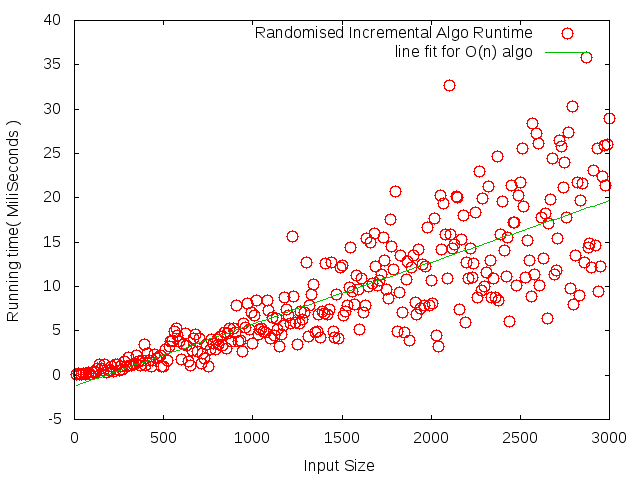
\includegraphics[width=0.5\columnwidth]{incr_loop1.png}%
\caption{Runtime vs Input Size plot for Randomised Incremental algorithm with linear fit. }
\label{fig:proto}%
\end{figure}
\textbf{Inference:} This plot, although is linear in general but as expected has significant devations from the line fit. Which is as expected since although its expected runtime is $O(n)$ but it can deviate from that because of its randomised nature depending on the order the points are processed by the algorithm. 
\newpage
\section*{Combined plot of the two Running time plots:}
\begin{figure}[th]%
\centering
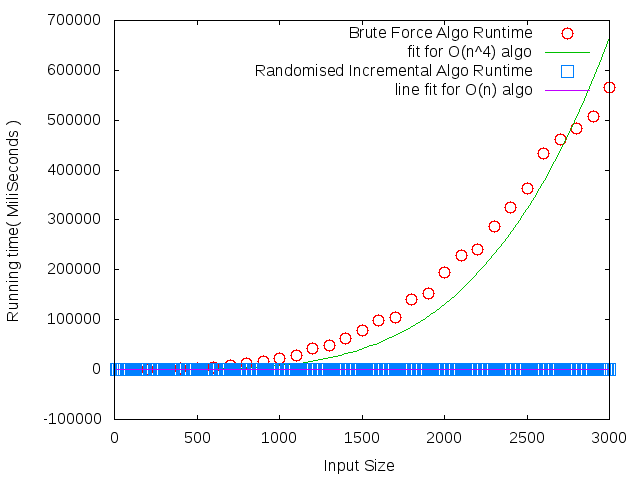
\includegraphics{combine_loop1.png}%
\hfill
\caption{Combined plot of the two Running time plots .}
\label{fig:proto}%
\end{figure}
\textbf{Inference:} We can see the huge difference of efficiency clearly in this plot as relative to the fast increase of the brute force running time the randomised algorithm runtime barely increases at all.
\newpage

\textbf{Note:} We have made a recursive implementation of the algorithm too. Looks like it is a bit slower than the loop(iterative) implementations because of function calling and function stack manipulations. Nevertheless its running time remains $O(n) = cn$ with a larger $c$, as can be seen in the plots shown below.

\section*{Running Time of Randomised Incremental algorithm(Recursive Implementation):}

\begin{figure}[th]%
\centering

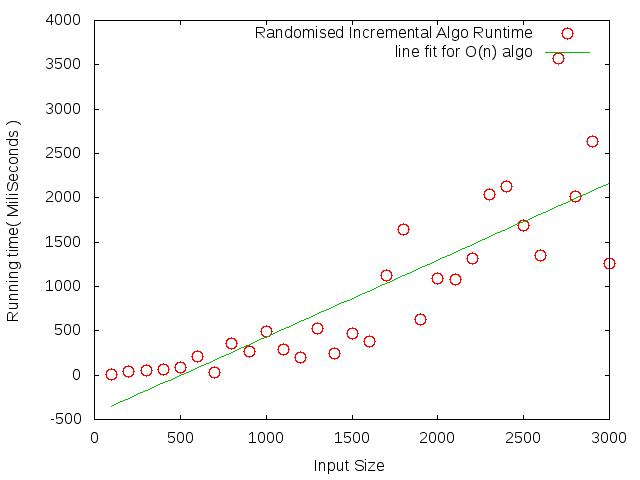
\includegraphics[width=0.5\columnwidth]{incr1.png}%
\caption{Runtime vs Input Size plot for Randomised Incremental algorithm with linear fit. }
\label{fig:proto}%
\end{figure}
\textbf{Inference:} This plot, although is linear in general but as expected has significant devations from the line fit. Which is as expected since although its expected runtime is $O(n)$ but it can deviate from that because of its randomised nature depending on the order the points are processed by the algorithm. 

\newpage

\section*{Combined plot of the Brute Force and O(n) Algo Recursive Implementation Running time plots:}

\begin{figure}[th]%
\centering
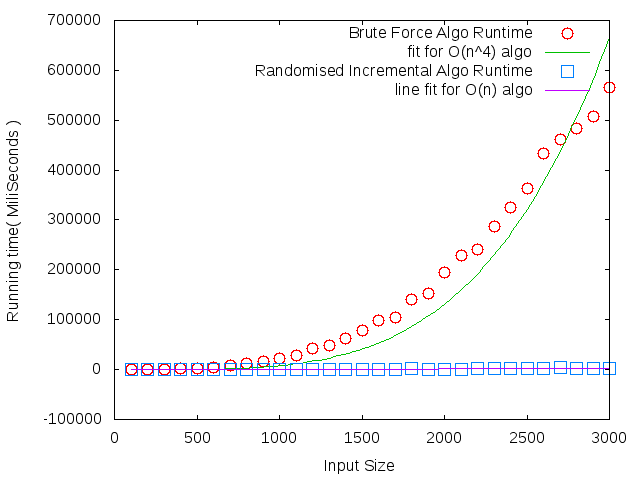
\includegraphics{combine1.png}%
\hfill
\caption{Combined plot of the two Running time plots .}
\label{fig:proto}%
\end{figure}


\newpage

\section*{Empirically found distribution of Randomised Algo:}

\subsection*{For Iterative Implementaion:}
	We ran our program with 10000 input size , 1000 times and plotted an histogram of the running times found for the iterative implementation. 
	
\begin{figure}[th]%
\centering
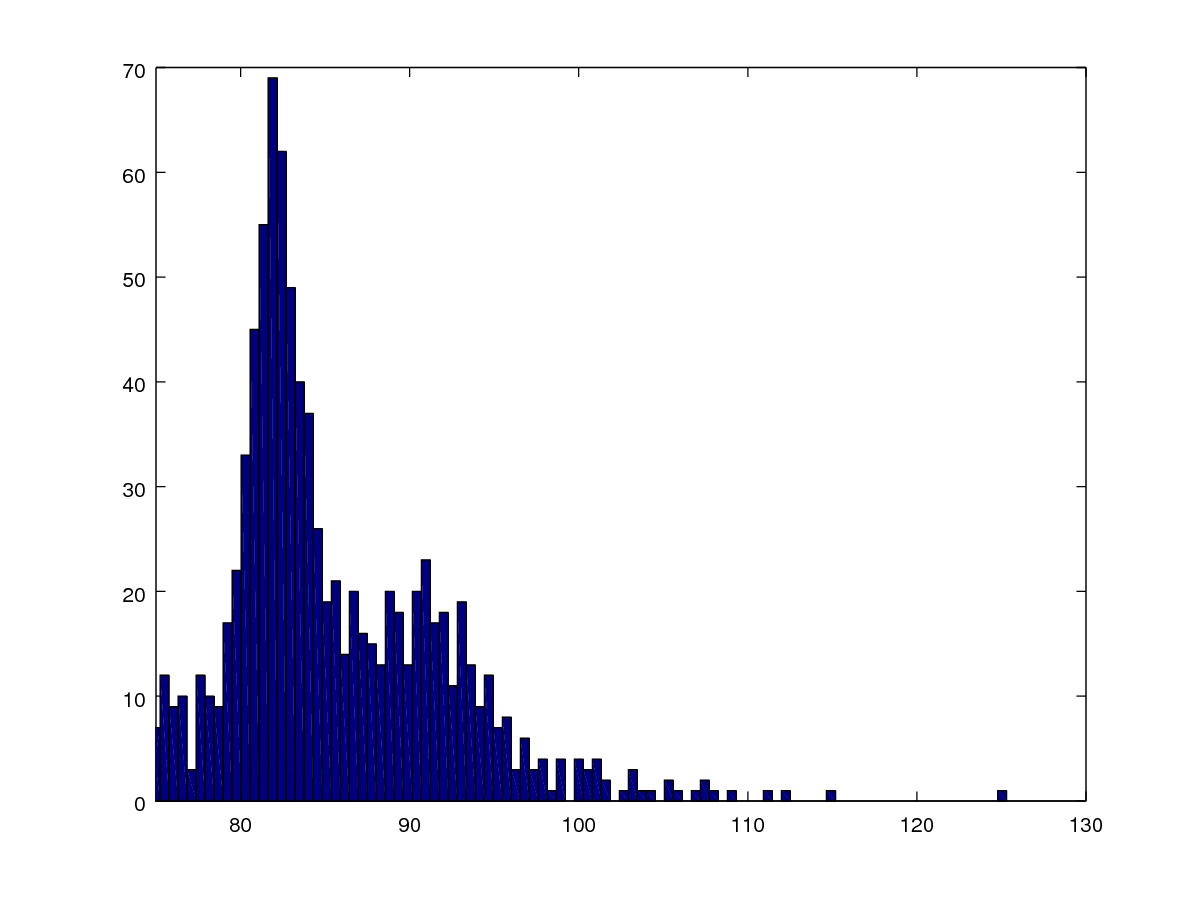
\includegraphics[width=0.8\columnwidth]{incrhist.png}%
\caption{Histogram showing distribution of runtimes of the randommised algorithm for input size 1000 for Iterative Implementation. }
\label{fig:proto}%
\end{figure}

\textbf{Inference:}

As shown, this looks like a normal distribution which is skewed to the left. Which is reasonable since although the expected(mean) runtime is O(n), it can shoot up to much higher values in cases.

Mean : 84.445 miliseconds
Standard Deviation : 7.0187 miliseconds
162 out of 1000 runs gave a higher runtime than mean + SD. Which gives a 16.2\% significant deviation. Coefficient of variability(SD/mean) is 0.083.\\

\newpage

\subsection*{For Recursive Implementation:}

We ran our program with 1000 input size , 1000 times and plotted an histogram of the running times found for the iterative implementation. 
	
\begin{figure}[th]%
\centering
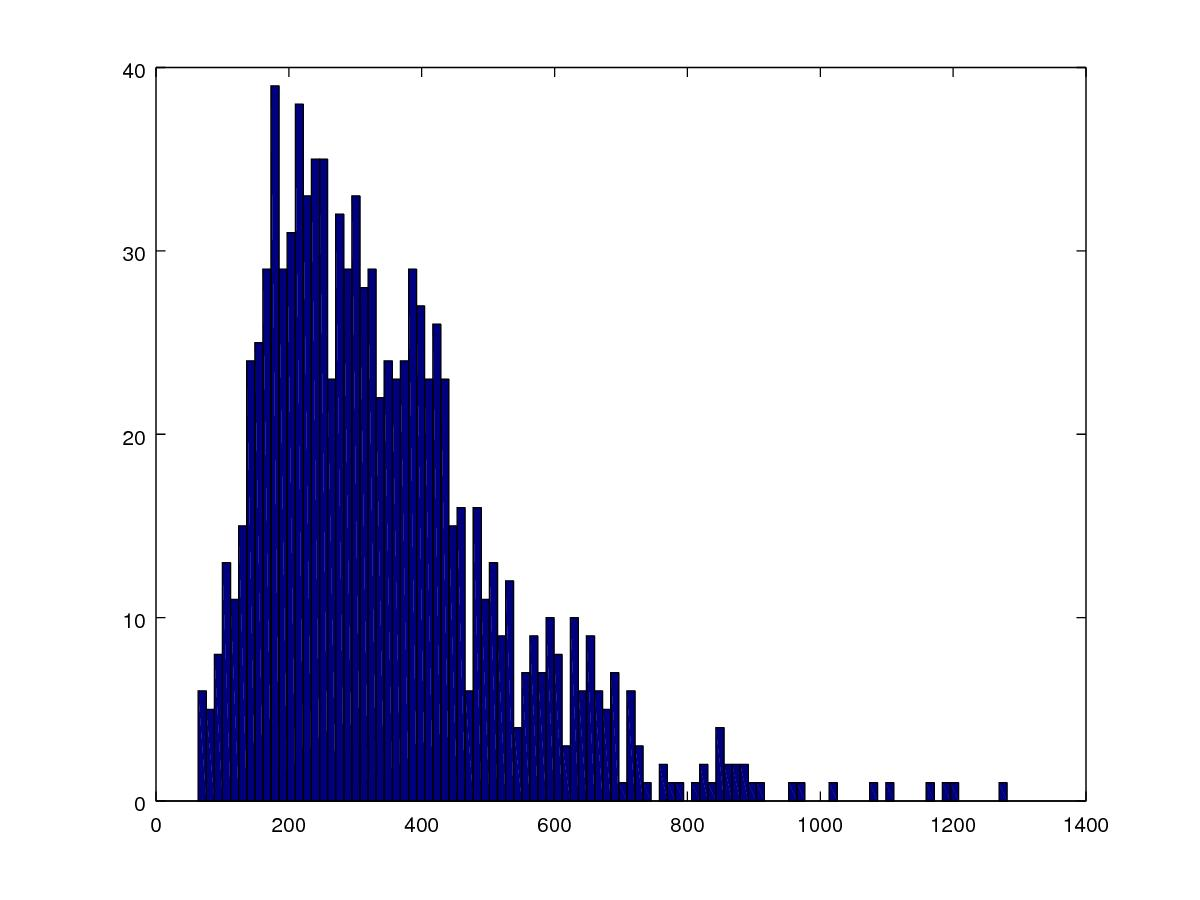
\includegraphics[width=0.8\columnwidth]{hist.jpg}%
\caption{Histogram showing distribution of runtimes of the randommised algorithm for input size 1000 for Iterative Implementation. }
\label{fig:proto}%
\end{figure}

\textbf{Inference:}

As shown, this looks like a normal distribution which is skewed to the left. Which is reasonable since although the expected(mean) runtime is O(n), it can shoot up to much higher values in cases.

Mean : 345.68 miliseconds
Standard Deviation : 179.32 miliseconds
144 out of 1000 runs gave a higher runtime than mean + SD. Which gives a 14.4\% significant deviation. Coefficient of variability(SD/mean) is 0.518.\\

\end{document}